\documentclass[10pt]{beamer}
\usetheme[numbering=fraction, background=light]{metropolis}

\usepackage{graphicx}
\usepackage{booktabs}
\usepackage{amsmath, amsthm, amssymb}

\title{Singularity of Magic Squares}
\subtitle{Investigation with Eigenvalues of Magic Squares}
\author{Elias Gee, Elijah Ecret, and Zih-Yu Hsieh}
\institute{UCSB, CCS Mathematics}
\date{\today}

\setbeamertemplate{theorems}[ams style]
%\newtheorem{theorem}{Theorem}
%\newtheorem{corollary}[theorem]{Corollary}
%%\newtheorem{definition}[theorem]{Definition}
%\newtheorem{example}[theorem]{Example}
%\newtheorem{lemma}[theorem]{Lemma}
\newtheorem{proposition}[theorem]{Proposition}
\newtheorem{remark}[theorem]{Remark}
\newtheorem{question}{Question}
\newtheorem{property}{Property}

\begin{document}

\maketitle

\begin{frame}{Outline}
    \tableofcontents
\end{frame}

\begin{frame}{References (\textbf{Need Detailed information)}}
\begin{enumerate}
    \item Even Order Regular Magic Squares are Singular - Bruce Mattingly, AMM, 107:9, 777-782
    \item On nonsingular regular magic squares of odd order, Lee, Love, Narayan
    \item Magic square spectra, Loly, Cameron, Trump, Schindel
    \item An investigation of even order magic squares (4, 6, 8): characteristic polynomials, eigenvalues, and encryption, Ashhab, Al-qdah
    \item To construct a magic square of order 2n from a given square of order n, Candy
    \item Self-complementary magic squares of singly even orders, Chia, Kok
\end{enumerate}
\end{frame}

\section{Introduction}

\begin{frame}{What is a Magic Square?}
    \begin{itemize}
      \item An $n\times n$ matrix with entries $1,...,n^2$
      \item Rows, columns, main diagonals add up to the same thing: $\mu=\frac{n^3+n}{2}$
    \end{itemize}
  
    \hfil
  
    \begin{example}A $4\times 4$ magic square with $\mu=\frac{4^3+4}{2}=34$.
    \[\begin{pmatrix}
      16&3&2&13\\
      5&10&11&8\\
      9&6&7&12\\
      4&15&14&1
    \end{pmatrix}\]
    \end{example}
  \end{frame}
  
  \begin{frame}{Regular Magic Square}
    \begin{definition}
      Entries $a,b$ are \emph{complements} if $$a+b=\frac{2\mu}{n} = n^2+1$$.
    \end{definition}
    \begin{definition}
      If all antipodal entries are complements, then the magic square is \emph{regular}.
    \end{definition}
  
    \begin{example}
    A $4\times 4$ magic square, $\mu=\frac{4^3+4}{2}=34$, $\frac{2\mu}{4}=17$.
    \[\left(\begin{array}{cc|cc}
      \textcolor{red}{16}&\textcolor{blue}{3}&2&13\\
      5&10&\textcolor{orange}{11}&\textcolor{cyan}{8}\\
      \midrule
      \textcolor{cyan}{9}&\textcolor{orange}{6}&7&12\\
      4&15&\textcolor{blue}{14}&\textcolor{red}{1}
    \end{array}\right)\]
    \end{example}
  \end{frame}

  \begin{frame}{Observation}
    \begin{example}
        MATLAB generated Magic Squares:
        \[A=\begin{pmatrix}
            8&1&6\\
            3&5&7\\
            4&9&2
          \end{pmatrix},\quad \det A=-360\]
          \[B=\begin{pmatrix}
            16&3&2&13\\
            5&10&11&8\\
            9&6&7&12\\
            4&15&14&1
          \end{pmatrix},\quad \det B=0\] 
    \end{example}   
  \end{frame}

  \begin{frame}{Conjecture}
    \begin{figure}[h!]
        \begin{center}
            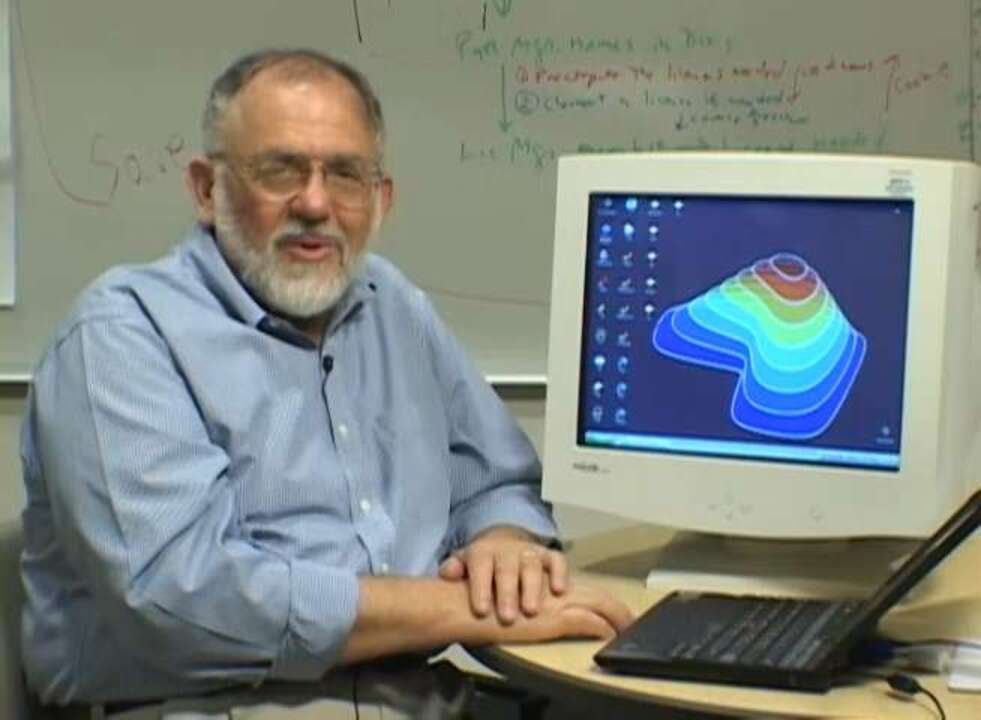
\includegraphics[width=60mm]{cleve moler.jpg}
            \caption{Cleve Moler, Creater of MATLAB}
        \end{center}
    \end{figure}

    \textbf{Cleve Moler's Conjecture:}
    \begin{itemize}
        \item Even Order magic squares are Singular 
        \item Odd Order magic squares are Nonsingular
    \end{itemize}
  \end{frame}

  \begin{frame}{Statement of Purpose}
    Collect and Compile known information about \textbf{Singularity of Magic Squares}.
  \end{frame}

\begin{frame}{Notation}
    \textbf{Define the following:}
    \[\mu = \textmd{Sum of each row, column, main diagonal}\]
    \[\textbf{e}=\begin{pmatrix}
    1\\1\\\vdots\\1\\1
    \end{pmatrix},\quad E=\begin{pmatrix}
        1&1&\cdots&1&1\\
        1&1&\cdots&1&1\\
        \vdots&\vdots&\ddots&\vdots&\vdots\\
        1&1&\cdots&1&1\\
        1&1&\cdots&1&1
    \end{pmatrix},\quad J=\begin{pmatrix}
        0&0&\cdots&0&1\\
        0&0&\cdots&1&0\\
        \vdots&\vdots&\ddots&\vdots&\vdots\\
        0&1&\cdots&0&0\\
        1&0&\cdots&0&0
    \end{pmatrix}\]
\end{frame}

\section{Even Order Regular Magic Squares are Singular - Bruce Mattingly, AMM, 107:9, 777-782} %Possibly need some examples

\begin{frame}{Methodology}
    Given $A$, Even Order Regular Magic Square.

    \textbf{Objective:} Prove that $0$ is an Eigenvalue of $A$.

    \textbf{Method:} Study matrices with similar spectra.
\end{frame}

\begin{frame}{Results}
    Given $A$ an Even Order Regular Magic Square:
    \begin{theorem}
        \begin{itemize}
            \item $A\textbf{e} = \mu\textbf{e}$, and $\textbf{e}^TA = \mu\textbf{e}^T$.
            \item $\mu$ as an eigenvalue of $A$, has multiplicity $1$.
        \end{itemize}
    \end{theorem}

    \hfil

    \begin{theorem}
        Let $Z=A-\frac{\mu}{n}E$, then:
        \begin{itemize}
            \item If $A\textbf{x}=\lambda\textbf{x}$ and $\lambda\neq \mu$, then $Z\textbf{x}=\lambda\textbf{x}$.
            \item $A\textbf{e} = \mu\textbf{e}$, and $Z\textbf{e}=\overline{0}$.
        \end{itemize}
    \end{theorem}
\end{frame}

\begin{frame}{Results}
    \begin{theorem}
        $Z$ is \textbf{skew-centrosymmetric}, i.e. $Z=-JZJ$. Which:
        \begin{itemize}
            \item If $Z\textbf{x}=\lambda\textbf{x}$, then $Z(J\textbf{x}) = -\lambda(J\textbf{x})$.
            \item Disregard signs, each eigenvalue $\lambda$ of $Z$ has even multiplicity.
            \item $0$ an eigenvalue of $Z$, has even multiplicity.
        \end{itemize}
    \end{theorem}
    
    \hfil

    \begin{theorem}
        Given $A$ an Even Order Regular Magic Square, then $0$ is an eigenvalue of $A$, $A$ is singular.
    \end{theorem}
\end{frame}

\section{Singularity Condition of Odd-Order Regular Magic Square}
\begin{frame}{Previous Results}
    \textbf{Recall:}
    \begin{itemize}
        \item If $A$ is a magic square, $\mu$ has multiplicity $1$
        \item If $A$ is regular, then $A+JAJ = \frac{2\mu}{n}E$.
        \item Define $Z:=A-\frac{\mu}{n}E$, then $Z=-JZJ$ (\textbf{Skew-centrosymmetric}).
        \item $Z$ inherits the spectra of $A$, except $\mu$ is swapped by $0$
    \end{itemize}
    EX:
    \[M_5 = \begin{pmatrix}
        11&24&7&20&3\\
        4&12&25&8&16\\
        17&5&13&21&9\\
        10&18&1&14&22\\
        23&6&19&2&15
    \end{pmatrix},\quad Z_5=\begin{pmatrix}
        \textcolor{red}{-2}&\textcolor{cyan}{11}&-6&\textcolor{orange}{7}&\textcolor{blue}{-10}\\
        -9&-1&12&-5&3\\
        4&-8&0&8&-4\\
        -3&5&-12&1&9\\
        \textcolor{blue}{10}&\textcolor{orange}{-7}&6&\textcolor{cyan}{-11}&\textcolor{red}{2}
    \end{pmatrix}\]
\end{frame}

%intro to new definitions required
\begin{frame}{Zero Magic Square}
    Given $A$ an $n\times n$ matrix, with $n^2$ distinct entries.
    \begin{definition}
        $A$ is a \textbf{Zero Magic Square}, if sum of each row, column, and main diagonal is $0$.
    \end{definition}

    \hfil

    EX: Any Magic Square $A$, $Z=A-\frac{\mu}{n}E$ is a zero magic square.
    \[A=\begin{pmatrix}
        16&3&2&13\\
        5&10&11&8\\
        9&6&7&12\\
        4&15&14&1
      \end{pmatrix},\quad Z=\begin{pmatrix}
        7.5&-5.5&-6.5&4.5\\
        -3.5&1.5&2.5&-0.5\\
        0.5&-2.5&-1.5&3.5\\
        -4.5&6.5&5.5&-7.5
      \end{pmatrix}\]
\end{frame}
\begin{frame}{Latin Squares}
    $A,\ B$ are $n\times n$ matrices.

    \begin{definition}
        $A$ is a \textbf{Latin Square}, if there are $n$ distinct entries.
        And, each entry appears once in each row and column.
    \end{definition}

    \begin{definition}
        $A,\ B$ are Latin Squares. The two are \textbf{Orthogonal}, if each pair of matched entries, $(a_{ij},b_{ij})$ is unique.
    \end{definition}

    \hfil

    EX:
    \[A=\begin{pmatrix}
        \textbf{0}&1&2\\1&2&\textcolor{red}{0}\\2&\textcolor{blue}{0}&1
    \end{pmatrix},\quad B=\begin{pmatrix}
        \textbf{0}&1&2\\2&0&\textcolor{red}{1}\\1&\textcolor{blue}{2}&0
    \end{pmatrix}\]
    \textbf{Observation:} $(0,0)$ appears only once.
\end{frame}
\begin{frame}{Circulant Matrices}
    \begin{definition}
        $A$ an $n\times n$ matrix is a \textbf{Circulant Matrix}, if for all $i<n$:
        $$\textmd{Row }i = \begin{pmatrix}
            a_1 & \cdots & a_{n-1} & a_n
        \end{pmatrix}$$
        $$\implies \textmd{Row }(i+1) = \begin{pmatrix}
            a_n & a_1 & \cdots & a_{n-1}
        \end{pmatrix}$$
    \end{definition}

    EX:
    \[B=\begin{pmatrix}
        \textcolor{red}{0}&1&2\\2&\textcolor{red}{0}&1\\1&2&\textcolor{red}{0}
    \end{pmatrix}\]
\end{frame}
\begin{frame}{Circulant Matrices}
    Let $S=\left\{\frac{-(n-1)}{2},...,-1,0,1,...,\frac{(n-1)}{2}\right\}$, and $\overline{a}=(a_1,...,a_n)$ contains all elements of $S$, with $a_1=0$.

    \begin{definition}
        $A$ an $n\times n$ circulant matrix, is $S$\textbf{-Circulant}, if row 1 of $A$ is some $\overline{a}$.
    \end{definition}

    EX: For $n=5$:
    \[A_{5}=\begin{pmatrix}
        0&2&-1&1&-2\\
        -2&0&2&-1&1\\
        1&-2&0&2&-1\\
        -1&1&-2&0&2\\
        2&-1&1&-2&0
    \end{pmatrix}\]
\end{frame}

%main condition theorem
\begin{frame}{Singularity Condition of Single-Order Regular Magic Square}
    Let $A$ be a $n\times n$ regular magic square, $n=2k+1$. Partition its $Z$ as:
    $$Z=\begin{pmatrix}
            Z_{11} & a & Z_{13}\\ b^T&0&-b^TJ\\ -JZ_{13}J & -Ja & -JZ_{11}J
        \end{pmatrix}$$
    Where $a,b\in\mathbb{R}^k$, and $Z_{11}, Z_{13}\in\mathbb{R}^{k\times k}$.

    \hfil

    \begin{theorem}
        $A$ is nonsingular, iff $(Z_{11}+Z_{13}J)$ and $(Z_{11}-Z_{13}J)$ are nonsingular.
    \end{theorem}
\end{frame}
\begin{frame}{Proof Sketch}
    \textbf{Goal:}

    Prove: $0$ not an eigenvalue of $A$ $\iff$ $0$ has multiplicity $1$ for $Z$

    $\iff$ $(Z_{11}+Z_{13}J)$, $(Z_{11}-Z_{13}J)$ are nonsingular.
\end{frame}
\begin{frame}{Proof Sketch}
    Let $Z'=K^{-1}ZK$ for specific $K$. Then:
    $$\det(Z'-\lambda I)=(-1)^k\lambda \det(C_{21}C_{12}-\lambda^2 I)$$
    $$C_{21}=\begin{pmatrix}
        Z_{11}-Z_{13}J\\2b^T
    \end{pmatrix},\quad C_{12}=\begin{pmatrix}
        (Z_{11}+Z_{13}J) & a
    \end{pmatrix}$$

    \hfil

    So, ($0$ has multiplicity $1$) $\iff$ ($\lambda^2$ not a factor)

    $\iff$ ($\det(C_{21}C_{12})\neq 0$)
\end{frame}
\begin{frame}{Proof Sketch}
    \[C_{21}C_{12}=(Z_{11}+Z_{13}J)(I+2E)(Z_{11}-Z_{13}J)\]
    \textbf{Note:} $(I+2E)$ is invertible.

    \hfil

    So, ($\det(C_{21}C_{12})\neq 0$) $\iff$ ($C_{21}C_{12}$ invertible)

    $\iff$ $(Z_{11}+Z_{13}J),\ (Z_{11}-Z_{13}J)$ are invertible.
\end{frame}

%Construction
\begin{frame}{Construction 1}
    Given $A$ an $n\times n$ matrix, $n$ odd.
    \begin{proposition}
        If $A$ is skew-centrosymmetric and $S$-circulant, let $Z=nA+AJ$.

        Then, $Z$ is a skew-centrosymmetric zero magic square, with entries
        $$\left\{\frac{-(n^2-1)}{2},...,-1,0,1,...,\frac{(n^2-1)}{2}\right\}$$
    \end{proposition}
\end{frame}
\begin{frame}{Construction 1}
    EX: $n=5$, $S=\{-2,-1,0,1,2\}$, and $\overline{a}=(0,2,-1,1,-2)$.
    \[A_{5}=\begin{pmatrix}
        0&2&-1&1&-2\\
        -2&0&2&-1&1\\
        1&-2&0&2&-1\\
        -1&1&-2&0&2\\
        2&-1&1&-2&0
    \end{pmatrix},\quad A_5J = \begin{pmatrix}
        -2&1&-1&2&0\\
        1&-1&2&0&-2\\
        -1&2&0&-2&1\\
        2&0&-2&1&-1\\
        0&-2&1&-1&2
    \end{pmatrix}\]
\end{frame}
\begin{frame}{Construction 1}
    \[Z_5 = nA_5+A_5J = 5\cdot A_5+A_5J\]
    \[=\begin{pmatrix}
        0&10&-5&5&-10\\
        -10&0&10&-5&5\\
        5&-10&0&10&-1\\
        -5&5&-10&0&10\\
        10&-5&5&-10&0
    \end{pmatrix} + \begin{pmatrix}
        -2&1&-1&2&0\\
        1&-1&2&0&-2\\
        -1&2&0&-2&1\\
        2&0&-2&1&-1\\
        0&-2&1&-1&2
    \end{pmatrix}\]
    \[=\begin{pmatrix}
        \textcolor{red}{-2}&\textcolor{blue}{11}&-6&7&-10\\
        -9&-1&12&\textcolor{orange}{-5}&\textcolor{cyan}{3}\\
        -4&-8&0&8&4\\
        \textcolor{cyan}{-3}&\textcolor{orange}{5}&-12&1&9\\
        10&-7&6&\textcolor{blue}{-11}&\textcolor{red}{2}
    \end{pmatrix},\quad rank(Z_5) = 4\]
\end{frame}

\begin{frame}{Construction 2} %need some other edits
    Suppose $A$ an $n\times n$ matrix, is skew-centrosymmetric, and $S$-circulant.
    \begin{proposition}
        \begin{itemize}
            \item If $n$ is an odd prime, then $rank(Z)=n-1$.
            \item If $n$ is an odd prime power, and the first row of $A$, $(a_1,...,a_n)$ has $a_i = i-1$ for $1\leq i\leq \frac{n-1}{2}$, then $rank(Z)=n-1$.
        \end{itemize}
    \end{proposition}
\end{frame}
\begin{frame}{Construction 3}
    EX: $n=5$
    \[A_{5}=\begin{pmatrix}
        0&2&-1&1&-2\\
        -2&0&2&-1&1\\
        1&-2&0&2&-1\\
        -1&1&-2&0&2\\
        2&-1&1&-2&0
    \end{pmatrix},\quad Z_5=\begin{pmatrix}
        -2&11&-6&7&-10\\
        -9&-1&12&-5&3\\
        -4&-8&0&8&4\\
        -3&5&-12&1&9\\
        10&-7&6&-11&2
    \end{pmatrix}\]
    \[M=Z_5 + \frac{\mu}{n}E = Z_5 + 13E\]
    \[ = \begin{pmatrix}
        -2&11&-6&7&-10\\
        -9&-1&12&-5&3\\
        -4&-8&0&8&4\\
        -3&5&-12&1&9\\
        10&-7&6&-11&2
    \end{pmatrix} + (13) = \begin{pmatrix}
        11&24&7&20&3\\
        4&12&25&8&16\\
        9&5&13&21&17\\
        10&18&1&14&22\\
        23&6&19&2&15
    \end{pmatrix}\]
    \[\det M=4,680,000\]
\end{frame}
\begin{frame}{Construction 3}
    Given $n$ odd prime power, $A$ an $n\times n$ skew-centrosymmetric $S$-circulant matrix.
    \begin{theorem}
        With $Z=nA+AJ$, then define:
        $$M=Z+\frac{\mu}{n}E = Z+\frac{n^2+1}{2}E$$
        $M$ is a Regular Magic Square, and $M$ is nonsingular.
    \end{theorem}
\end{frame}

\section{Centrosymmetric and Skew-centrosymmetric Matrices and Regular Magic Squares}
\begin{frame}{(Skew) Centrosymmetric Matrices}
    centro = center
\end{frame}

\begin{frame}{Spectra of Certain Matrices}
    \begin{itemize}
        \item $H$ = real centrosymmetric matrix
        \item $S$ = real skew-centrosymmetric
        \item $H+iS$ real eigenvalues
    \end{itemize}
    eigenvalues of $H\pm iS, H\pm JS$
    \\
    corresponding eigenvectors too
\end{frame}

\begin{frame}{Equivalence Between Symmetric Skew-Centrosymmetric and Doubly Skew Matrices}
    \begin{itemize}
        \item Eigenvalues
        \item Determinant
        \item Inverse
    \end{itemize}
\end{frame}

\begin{frame}{Takeaways from this Paper}
    \begin{itemize}
        \item Symmetries
        \item Equivalences
        \item Spectra
    \end{itemize}
\end{frame}

\section{Conclusion}




%\section{Conclusion}
\end{document}
